\chapter{Prezentacja warstwy użytkowej projektu}

\section{Warstwa Użytkowa Projektu}

Projekt Systemu Zarządzania Parkingiem oferuje intuicyjny i prosty w obsłudze interfejs użytkownika, który umożliwia szybkie zarządzanie miejscami parkingowymi oraz monitorowanie dostępności przestrzeni parkingowej. Interfejs użytkownika został zaprojektowany z myślą o zapewnieniu maksymalnej użyteczności i dostępności funkcji.

Aplikacja umożliwia użytkownikom wykonanie następujących akcji:
\begin{itemize}
    \item Sprawdzenie dostępności miejsc parkingowych.
    \item Rejestracja wjazdu i wyjazdu pojazdów.
    \item Zarządzanie danymi pojazdów.
\end{itemize}

Interfejs skupia się na minimalizmie i łatwości nawigacji, co pozwala na szybkie odnalezienie potrzebnych informacji i funkcji.

W tej sekcji zostaną umieszczone zrzuty ekranu przedstawiające kluczowe funkcjonalności aplikacji oraz jej interfejs użytkownika.

\begin{figure}[H]
\centering
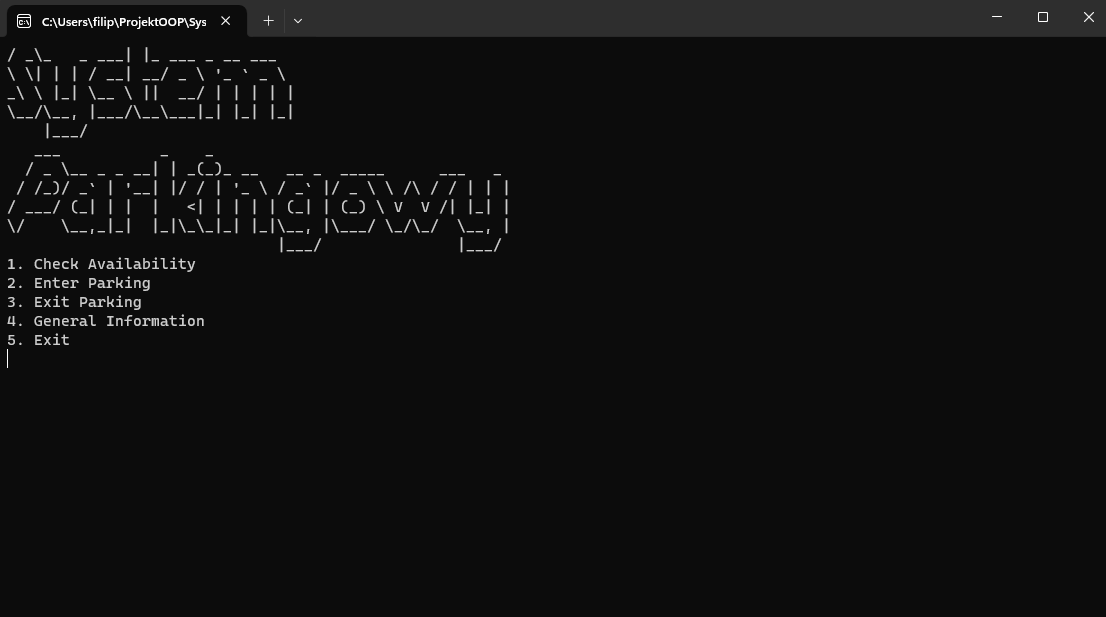
\includegraphics[width=\textwidth]{photos/mainmenu.png}
\caption{Widok głównego menu aplikacji.}
\end{figure}

W tej sekcji omówione zostaną kluczowe funkcjonalności aplikacji Systemu Zarządzania Parkingiem oraz instrukcje dotyczące ich używania.

\begin{itemize}
    \item \textbf{Sprawdzanie dostępności miejsc parkingowych} (\textit{Check Availability}):
    Użytkownik może sprawdzić dostępność miejsc parkingowych dla samochodów, wybierając opcję "1". 

    \begin{figure}[H]
    \centering
    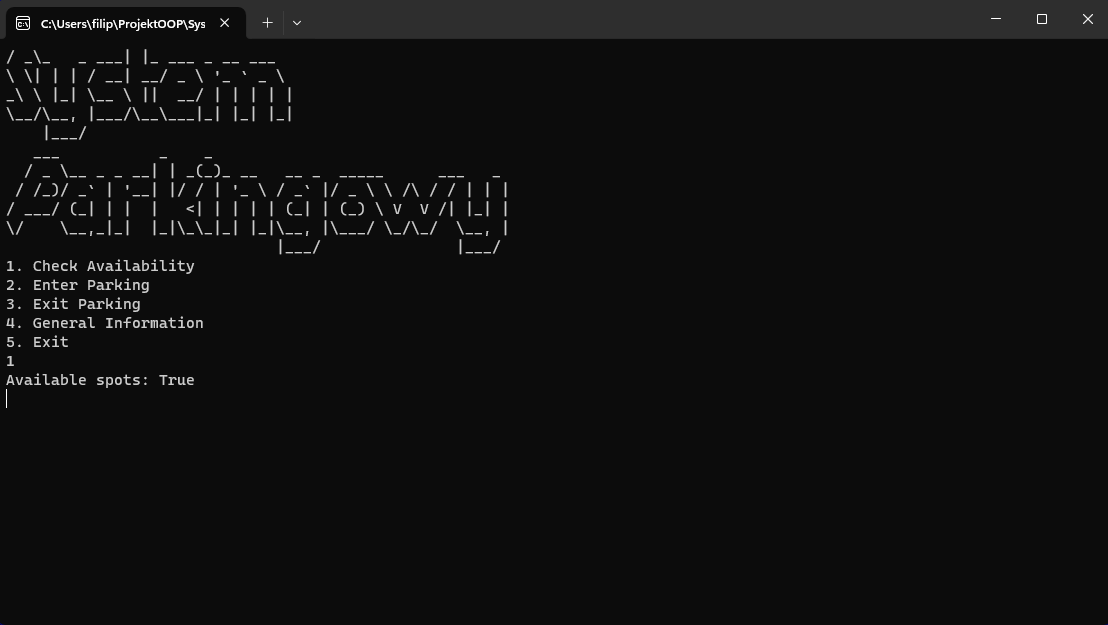
\includegraphics[width=\textwidth]{photos/avail.png}
    \caption{Opcja 1 - Check Availability.}
    \end{figure}

    \item \textbf{Wprowadzanie pojazdów na parking}:
    Użytkownik może wprowadzić pojazd na parking, wybierając opcję "2". Następnie należy podać numer rejestracyjny pojazdu, jego kolor oraz wybrać typ pojazdu (1 - Samochód, 2 - Motocykl, 3 - Autobus). Na podstawie podanych informacji, system tworzy odpowiedni obiekt pojazdu i rejestruje go w systemie parkingowym. 
        \begin{figure}[H]
        \centering
        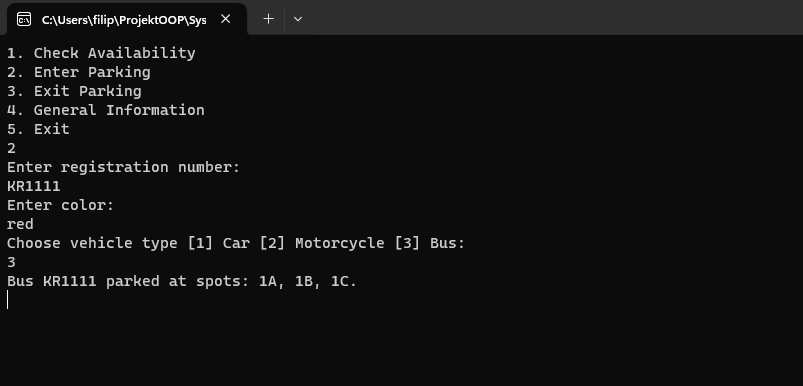
\includegraphics[width=\textwidth]{photos/enter.png}
        \caption{Opcja 2 - Enter Parking.}
        \end{figure}
    \clearpage
    \item \textbf{Wyjazd pojazdów z parkingu}:
    Użytkownik może wyjechać pojazdem z parkingu, wybierając opcję "3". Następnie należy podać numer rejestracyjny pojazdu. Na podstawie podanej informacji, system usuwa pojazd z rejestru parkingowego. 
    \begin{figure}[H]
        \centering
        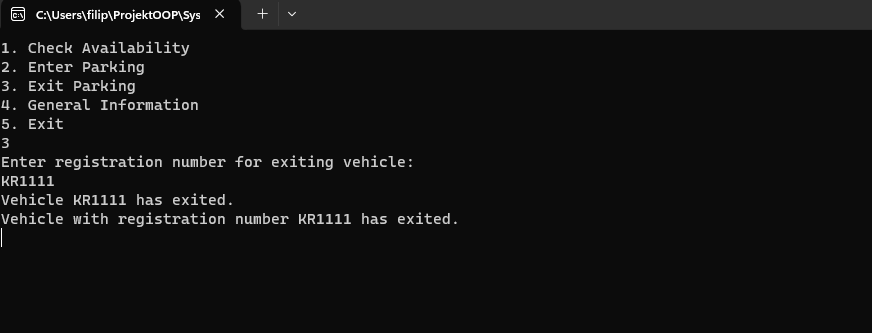
\includegraphics[width=\textwidth]{photos/exit.png}
        \caption{Opcja 3 - Exit Parking.}
        \end{figure}
    \item \textbf{Dodatkowe informacje}:
    Użytkownik wybierając opcję "4"\ wyświetla dodatkowe informacje o systemie.
        \begin{figure}[H]
        \centering
        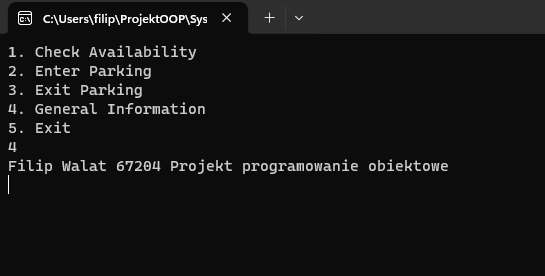
\includegraphics[width=\textwidth]{photos/info.png}
        \caption{Opcja 4 - General Information.}
        \end{figure} 
\item \textbf{Koniec}:
    Użytkownik wybierając opcję "5"\ zamyka aplikacje.
\end{itemize}
\clearpage
\section{Opis interakcji z użytkownikiem}
Sekcja ta zawiera informacje na temat interakcji z użytkownikiem, w tym otrzymywanych komunikatów, alertów oraz sposobu obsługi błędów. Poniżej przedstawiono wybrane komunikaty wyświetlane przez aplikację:

\begin{itemize}
    \item \texttt{"Available spots: [True lub False]"} - informacja mówiąca czy znajdują się obecnie wolne miejsca parkingowe.
    \item \texttt{"Enter registration number:"} - monit o wprowadzenie numeru rejestracyjnego pojazdu.
    \item \texttt{"Enter color:"} - prośba o podanie koloru pojazdu.
    \item \texttt{"Choose vehicle type [1] Car [2] Motorcycle [3] Bus:"} - wybór typu pojazdu do wprowadzenia na parking.
    \item \texttt{"Invalid vehicle type selected."} - komunikat o błędnym wyborze typu pojazdu.
    \item \texttt{"Vehicle entered the parking."} - informacja o pomyślnym wprowadzeniu pojazdu na parking.
\end{itemize}
